\chapter{Combining RL and Auto-regression}
\label{chap:RL-Autoregression}

How can we combine reinforcement learning with auto-regressive learning?

\begin{equation}
	\vcenter{\hbox{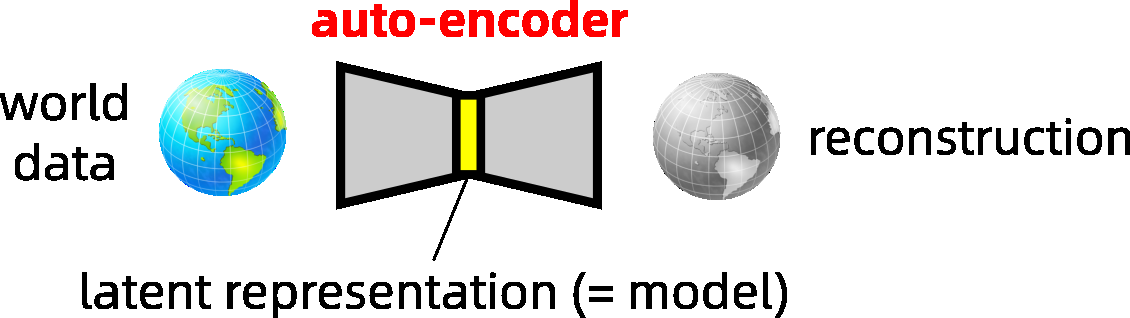
\includegraphics[scale=0.7]{auto-encoder.png}}}
\end{equation}

\begin{itemize}
	\item world = state, basically
	\item world $\subset$ state or world $\supset$ state ?
\end{itemize}

\begin{equation}
% from /2023/RL-with-world-model.svg and generative-models-and-AGI.svg
\vcenter{\hbox{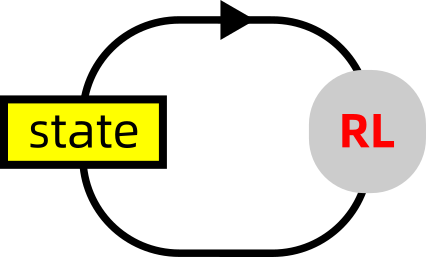
\includegraphics[scale=0.7]{minimal-RL.png}}}
\qquad \qquad
\vcenter{\hbox{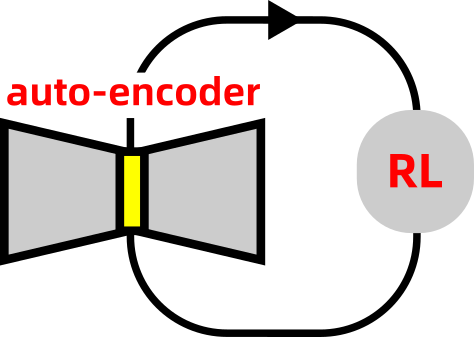
\includegraphics[scale=0.7]{RL-with-autoencoder.png}}}
\end{equation}

If we use RL to model internal mental states, then each action is an internal next thought.  In this setting, what does auto-regression, or ``prediction of the next state,'' mean?

Perhaps think about the example of Tic-Tac-Toe:
\begin{equation}
\vcenter{\hbox{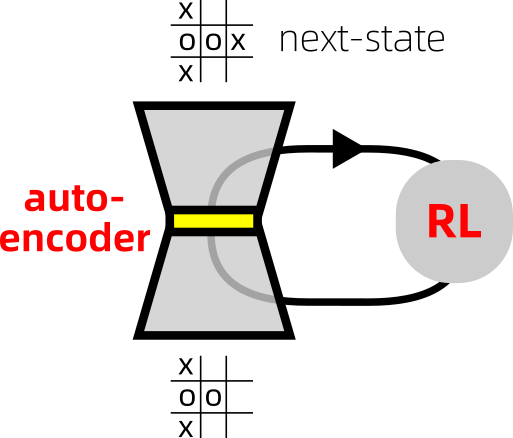
\includegraphics[scale=0.7]{RL-with-autoencoder-TTT.png}}}
\end{equation}
What we call ``prediction'' should be about external world-states.  

Think about it:  it does not make too much sense for auto-regression to predict the next \textit{internal} thought;  that would be highly redundant.



\begin{equation}
\vcenter{\hbox{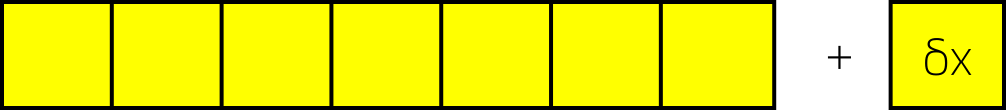
\includegraphics[scale=0.7]{state-with-delta.png}}}
\end{equation}


